% Data flow diagram
% Author: David Fokkema
\documentclass{article}
\usepackage{tikz}
\usetikzlibrary{shapes,arrows}
\usepackage{pdflscape}
\usepackage[papersize={7cm, 7.3cm}, text={7cm, 7.3cm}]{geometry}
\usetikzlibrary{decorations.text}
\usepackage{xcolor}
% \selectcolormodel{gray}

\begin{document}
\thispagestyle{empty}
%\begin{landscape}
\begin{center}
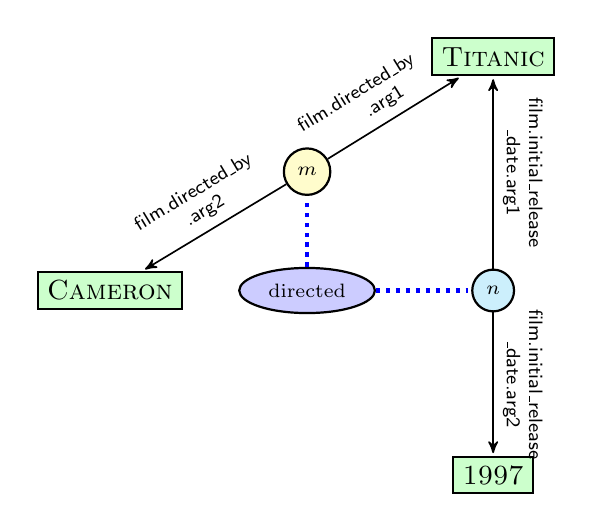
\begin{tikzpicture}[
  font=\sffamily,
  every matrix/.style={ampersand replacement=\&,column sep=0.7cm,row sep=0.9cm,font=\scriptsize},
  entity/.style={draw,thick,rectangle,fill=green!20,font=\sc},
  word/.style={draw,thick,ellipse,fill=blue!20},
  mediator/.style={draw,thick,circle},
  mediatorR/.style={draw,thick,circle,fill=cyan!20},
  mediatorV/.style={draw,thick,circle,fill=violet!20},
  mediatorY/.style={draw,thick,circle,fill=yellow!20},
  entityType/.style={draw,thick,rounded corners,fill=yellow!20,inner sep=.3cm},
  mathType/.style={draw,thick,diamond,fill=red!20},
  mediatorToEntity/.style={->,>=stealth',shorten
>=1pt,semithick,black,sloped,above,font=\sffamily\scriptsize},
  typeToEntity/.style={->,>=stealth',shorten >=1pt,semithick,black,sloped,above,font=\sffamily\scriptsize},
  wordToEntity/.style={-,>=stealth',shorten >=1pt,ultra
thick,dotted,blue,sloped,above,font=\sffamily\scriptsize},
  entityToMath/.style={->,>=stealth',shorten >=1pt,ultra
thick,dashed,violet,sloped,above,font=\sffamily\scriptsize},
  every node/.style={align=center}]

  % Cameron directed Titanic in 1997.
  
  % Position the nodes using a matrix layout
  \matrix{ 
    \&  \& \node[entity] (eTitanic) {Titanic}; \\
    \& \node[mediatorY] (m1) {$m$}; \&  \\
    \node[entity] (eCameron) {Cameron}; \& \node[word] (wDirected)
{directed}; \& \node[mediatorR] (m2) {$n$};
\\
     \&  \&  \\
     \&  \& \node[entity] (e1997) {1997}; \\
  };
 
  % words to entities
  % \draw [wordToEntity] (wCameron) edge node {}  (eCameron);
  % \draw [wordToEntity] (wTitanic) edge node {}  (eTitanic);
  % \draw [wordToEntity] (w1997) edge node {}  (e1997);
  
  % event word to mediators
  \draw [wordToEntity] (wDirected) edge node {}  (m1);
  \draw [wordToEntity] (wDirected) edge node {}  (m2);
  % \draw [wordToEntity] (wDirected) edge node {}  (m3);
  
  % mediator to entities
  \draw [mediatorToEntity] (m1) edge node {film.directed\_by\\.arg2}  (eCameron);
  \draw [mediatorToEntity] (m1) edge node {\hspace{-0.5cm}film.directed\_by\\.arg1}  (eTitanic);
  
  \draw [mediatorToEntity] (m2) edge node {film.initial\_release\\\_date.arg2}  (e1997);
  \draw [mediatorToEntity] (m2) edge node[rotate=180] {film.initial\_release\\\_date.arg1} 
(eTitanic);
  
  % \draw [mediatorToEntity] (m3) edge node {directed.arg1}  (eCameron);
  % \draw [mediatorToEntity] (m3) edge node {directed.in}  (e1997);
 
  
\end{tikzpicture} 
\scriptsize $\mbox{film.directed\_by.arg2}(m, \textsc{Cameron})$ $\wedge$ 
$\mbox{film.directed\_by.arg1}(m, \textsc{Titanic}) \wedge
\mbox{film.initial\_release\_date.arg1}(n,
\textsc{Titanic}) \wedge \mbox{film.initial\_release\_date.arg2}(n, \textsc{1997})$
\end{center}
 
% \end{landscape}

% \begin{tikzpicture}
% \node (One) at (-3,0) [shape=circle,draw] {$One$}; 
% \node (Two) at (3,0) [shape=circle,draw] {$Two$};
% \def\myshift#1{\raisebox{-2.5ex}}
% \draw [->,thick,postaction={decorate,decoration={text along path,text
% align=center,text={|\sffamily\myshift|Some more bent text}}}] (One) to [bend right=45]  (Two);
% \def\myshift#1{\raisebox{1ex}}
% \draw [->,thick,postaction={decorate,decoration={text along path,text
%align=center,text={|\sffamily\myshift|Some bent text}}}]      (One) to [bend left=45] (Two);
% \end{tikzpicture}


\end{document}
